\chapter{Introduction}
The flow around circular cylinders has become an important research field. In recent years, this kind of problems are increasingly appearing in biology, medical science and chemistry, waiting for people's further research.


\section{Flow Around Circular Cylinders}
The flow past a bluff body is of importance in both the nature and engineering practice. Ships run on the surface of water, aircrafts navigate the air, the river flows through the bridge, the sea around the island, and the wind blows over tall buildings. These are all the examples of the flow past a bluff body, which can be observed in every corner of the world, and are closely linked with our life.

Flow around circular cylinders is an classical problem in fluid mechanics. The flow state can be divided into several stage\cite{zdravkovich1997flow}. In domain far from the cylinder, the flow can be described with potential flow theory. In domain near the cylinder, the flow can be divided into four parts, as shown in Figure \ref{fig: flow area}. This four 
\begin{figure}
	\centering
	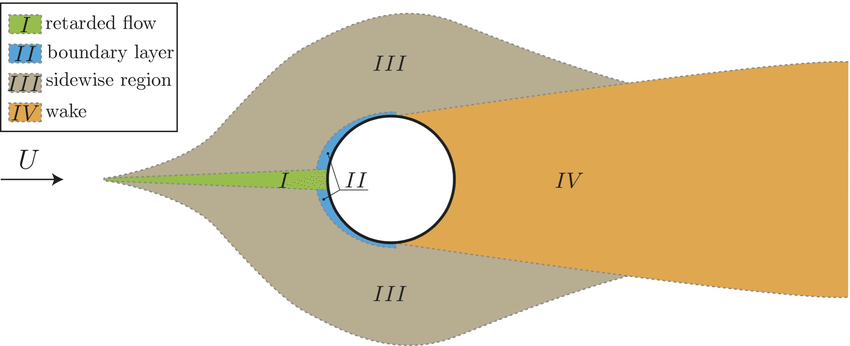
\includegraphics[scale=.4]{figs/Regions-of-disturbed-flow-around-a-perfect-circular-cylinder}
	\caption{The division of the flow area.}\label{fig: flow area}
\end{figure}


\section{Flow Through Porous Medium}
\section{Flow past and Through Porous Bluff Bodies}
\section{Research Question and Dissertation Structure Arrangement}
